\documentclass[a4paper,french]{paper}
\usepackage{../../_latex_assets/villemejane_iogs_ceti}

%Informations about this document 
%------------------------------------------
\def\module{Conception Electronique pour le Traitement de l'Information}
\def\moduleAbrege{5N-027-SCI / CéTI}
\def\annee{}

\def\titre{Bloc 2 / Filtrage actif}
\author{Julien VILLEMEJANE}

\subtitle{Bloc 2}
\institution{LEnsE / Institut d'Optique Graduate School}

\title{\titre}
\begin{document} 
%Beginning First Page. 
%------------------------------------------
\enteteThematiqueObligatoire{}

%Beginning Content. 
%------------------------------------------

\vspace{-1cm}
%%%%%%%%%%%%%%%%%%%
\encadreTDExo{2.1 - Filtrer des composantes fréquentielles - Ordre 1 Passif}{
Proposer une structure de filtre du premier ordre qui laisse passer des signaux au dessus d'une fréquence $f_c$. Donner les principales caractéristiques et limitations d'un tel filtre.
}


%%%%%%%%%%%%%%%%%%%
\encadreTDExo{2.2 - Filtrer des composantes fréquentielles - Ordre 2}{
On se propose d'étudier la structure suivante :

\begin{center}
	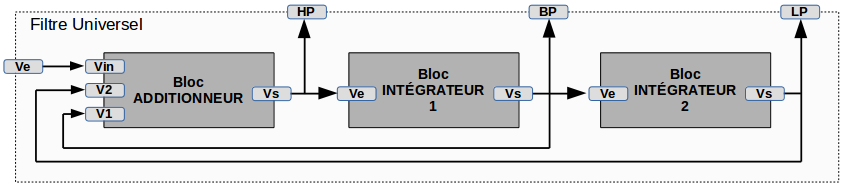
\includegraphics[width=14cm]{images/universel_structure.png}
\end{center}

Pour cela, on se propose d'étudier les deux circuits suivants :

\begin{center}
	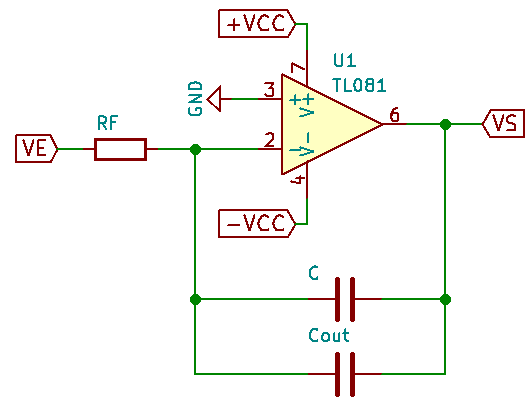
\includegraphics[width=7cm]{images/universel_integrateur.png}
	\quad
	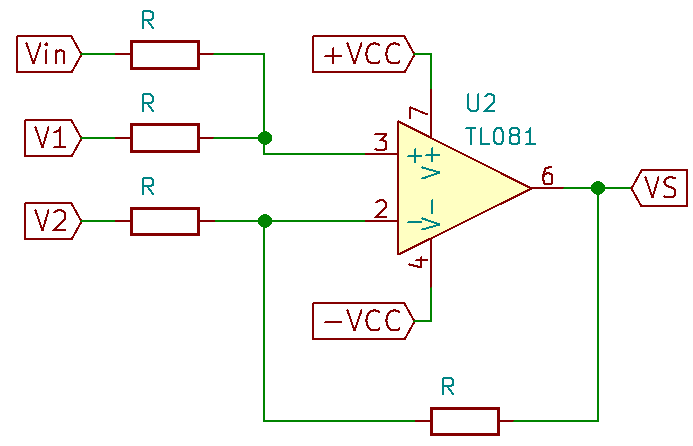
\includegraphics[width=7cm]{images/universel_sommateur.png}
\end{center}
}

\encadreTDExo{2.4 - Réaliser un filtre à partir d'un gabarit}{
On s'intéresse ici aux filtres de \textbf{Butterworth} (voir annexe). 

On souhaite réaliser un filtre dont le gabarit est le suivant :

\begin{itemize}
	\item gain supérieur à $-1\operatorname{dB}$ jusqu'à $10\operatorname{kHz}$
	\item gain inférieur à $-60\operatorname{dB}$ à partir de $40\operatorname{kHz}$
\end{itemize}

\bigskip

\begin{enumerate}
	\item Tracer le gabarit du filtre.
	\item Déterminer l'ordre du filtre minimal.
	\item Déterminer la pulsation de coupure du filtre.
	\item Déterminer la fonction de transfert du filtre	
\end{enumerate}

}

%%%%%%%%%%%%%%%%%%%
\encadreTDExo{2.3 - Filtrer des composantes fréquentielles autrement}{

\subsection*{Capacité commutée}

On se propose d'étudier la structure suivante, dont l'interrupteur $K$ est piloté par le signal de commande ci-dessous :

\begin{center}
	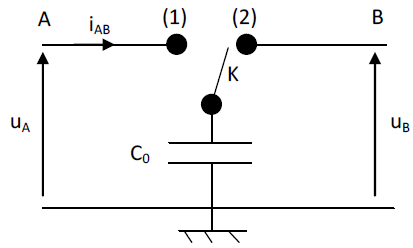
\includegraphics{images/capa_comm.png} 
	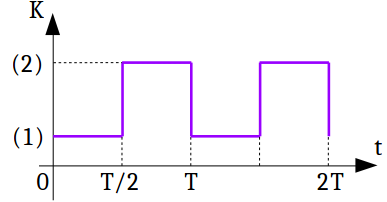
\includegraphics{images/capa_comm_signal.png}
\end{center}

\medskip

\begin{enumerate}
	\item Calculer la charge stockée dans $C_0$ entre les instants 0 et $T/2$, puis entre les instants $T/2$ et $T$.
	\item Quelle quantité de charges passe de A vers B entre les instants 0 et T ?
	\item Calculer alors le courant moyen circulant du point A au point B pendant une période T. 
	\item Donner l'expression de la résistance équivalente $R_{AB}$ vue entre les bornes A et B de cette cellule.
\end{enumerate}

\subsection*{Intégrateur}

On réalise un intégrateur à partir du circuit de la figure 2.

\begin{enumerate}
	\item Donner la fonction de transfert du circuit $T(j\omega) = u_2/u_1$ en fonction de $R_{AB}$ et de $C$.

\begin{center}
	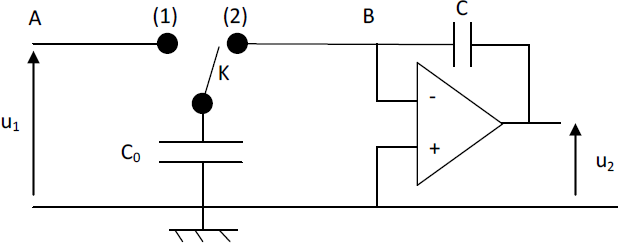
\includegraphics{images/capa_comm_integrateur.png}
\end{center}

	\item Que devient alors la fonction de transfert $T(j\omega{}) = u_2/u_1$ en fonction des éléments du système ($C_0$ et $C$) ?
	\item Quel est l'intérêt d'un tel circuit ?
\end{enumerate}

\subsection*{Etude du MAX296}

On s'intéresse au composant MAX296 dont une partie de la documentation technique est donnée en annexe.

\begin{enumerate}
	\item Quelles sont les fréquences maximales utilisables sur l'entrée \textsc{INPUT} ? Sur l'entrée \textsc{CLOCK} ? Quelles sont les applications visées ?
	\item Quelle fréquence faut-il appliquer sur l'entrée \textsc{CLOCK} pour avoir une fréquence de coupure de 3~kHz ? Que vaut alors l'amplification théorique du signal à : (a) 300~Hz ? (b) 30~kHz ? (c) 5~kHz ?
	\item Avec un filtre du second ordre (type Rauch) avec une pulsation de coupure à la même valeur, quelle aurait été l'amplification : (a) à 30~kHz ? (b) à 5~kHz ?	
	
\end{enumerate}

}

%%%%%%%%%%%%%%%%%%%

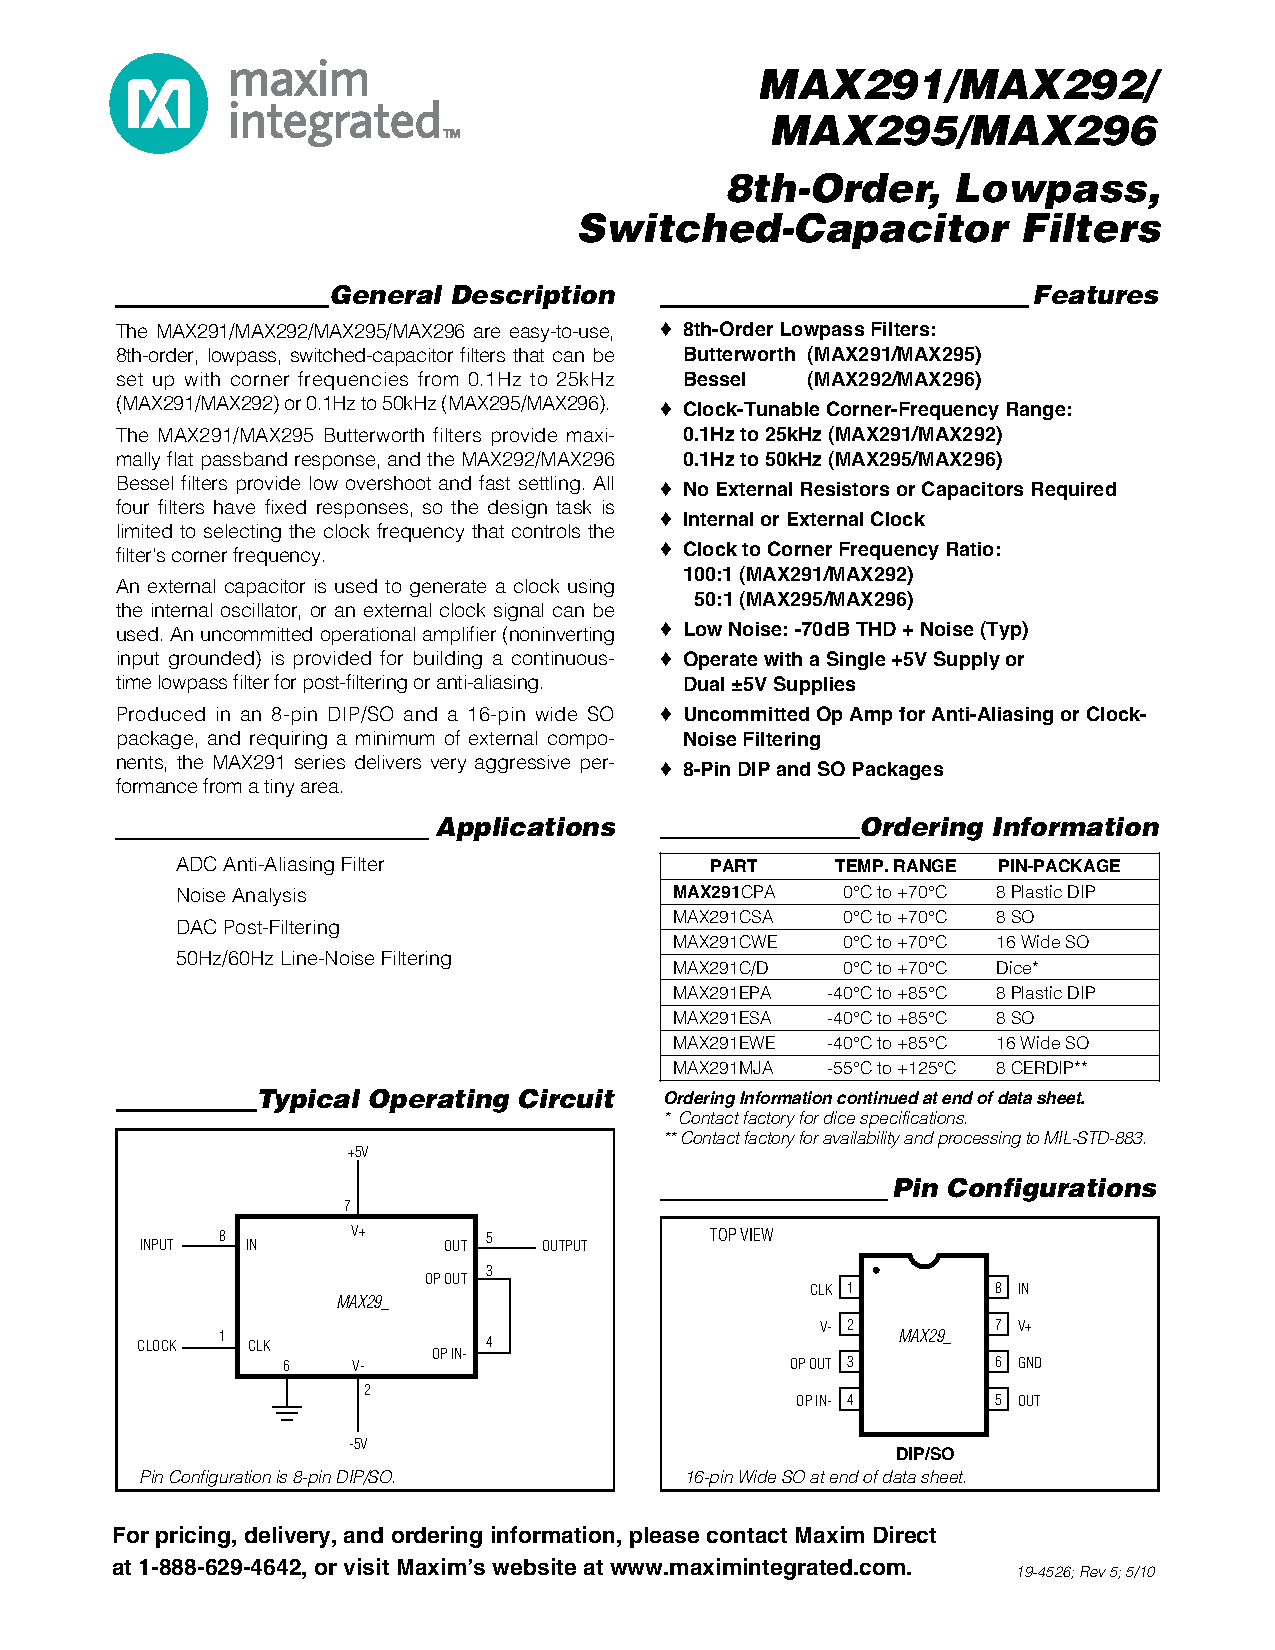
\includepdf[pages=-]{doc/MAX296.pdf}

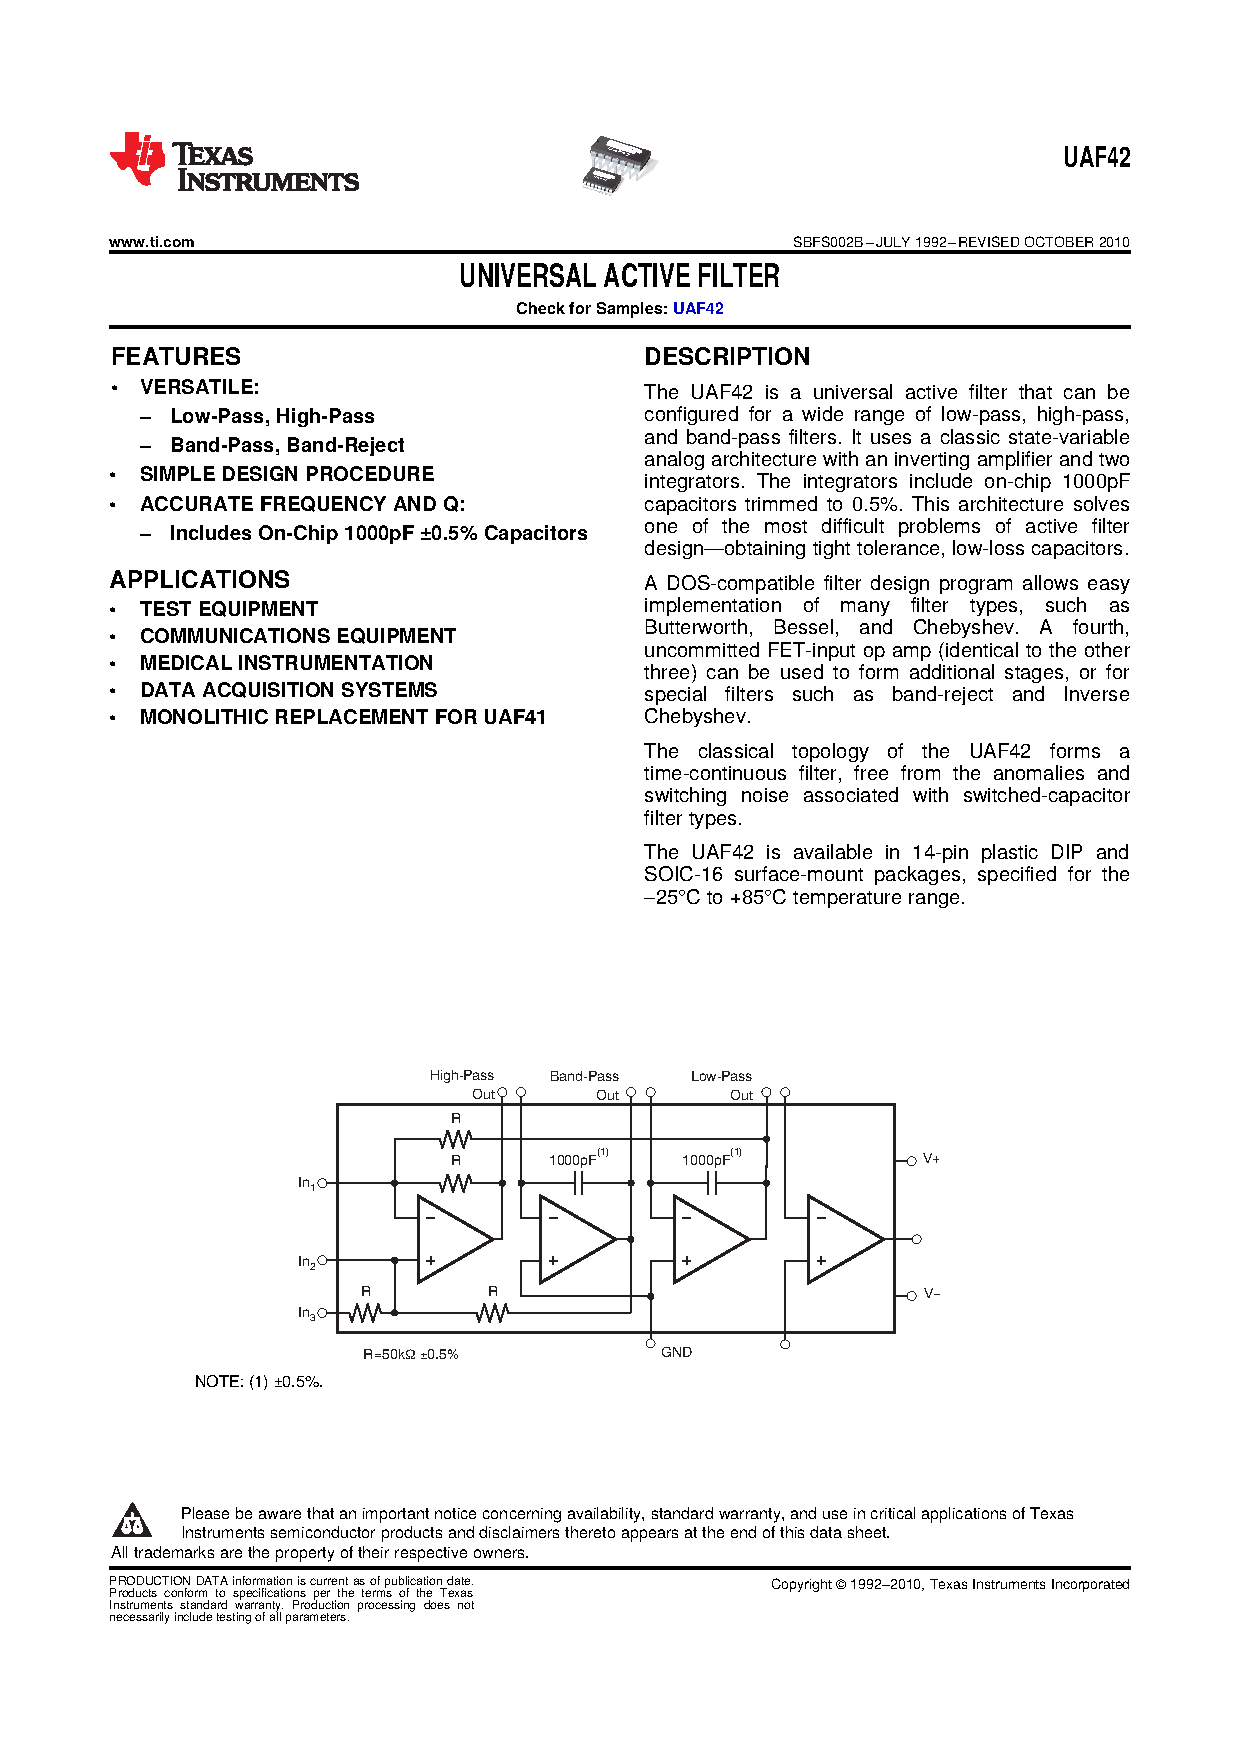
\includepdf[pages=-]{doc/uaf42.pdf}

\newpage
\section*{Annexe : Filtres actif de \textbf{Butterworth} et de \textbf{Chebychev}}

\textit{Document basé sur le cours de Sylvie Lebrun, Filtrage analogique, 2015.}

\subsection*{Gabarit d'un filtre}

Le gabarit d'un filtre correspond aux \textbf{contraintes fréquentielles et en gain} que doit satisfaire le système à développer.

\begin{center}
	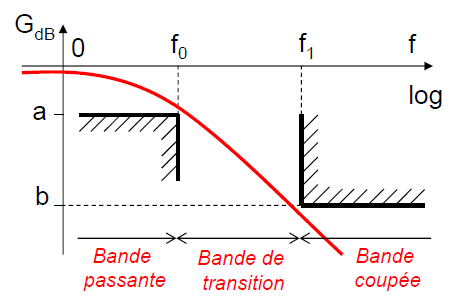
\includegraphics[width=10cm]{images/gabarit_filtre.png}
\end{center}

On souhaite souvent réaliser un système de filtrage qui possède les caractéristiques suivantes :
\begin{itemize}
	\item transmission de fréquence inférieure à $f_0$
	\item valeur minimale $a$ de gain dans la bande de fréquence à transmettre
	\item valeur maximale $b$ de gain dans la bande de fréquence à éliminer (à partir d'une fréquence $f_1$)
\end{itemize}

Le gabarit est caractérisé par 2 points $(f_0, a)$ et $(f_1, b)$.

\medskip

A partir de ce gabarit, plusieurs types de filtres peuvent être utilisés : Butterworth, Chebychev, Bessel, Cauer

\bigskip

Pour la suite, on posera : $X = \frac{\omega}{\omega_c}$ où $\omega_c$ est la fréquence de coupure du système, définie à $-3\operatorname{dB}$ par rapport au gain dans la bande passante.


\begin{center}
	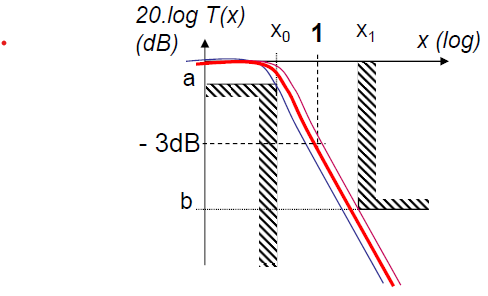
\includegraphics[width=8cm]{images/gabarit_butter.png}
\end{center}

\newpage
\subsection*{Filtre de Butterworth}

Ce type de filtre est utilisé pour sa \textbf{réponse extrêmement plate dans la bande-passante}.


La réponse en fréquence d'un tel filtre est tel que son module vaut :

$$ T(X) = \frac{1}{\sqrt{1 + X^{2\cdot n}}}$$

où $n$ est l'ordre du filtre.

\subsubsection*{Détermination de $n$}
En s'intéressant aux conditions aux limites :


$
\left\{
    \begin{array}{ll}
        20 \cdot \log_{10} T(x_0) > a \\
        20 \cdot \log_{10} T(x_1) < b \\
    \end{array}    
\right. 
$
$\Leftrightarrow$
$
\left\{
    \begin{array}{ll}
        x_0^{2\cdot n} < 10^{-a/10} - 1 & (1)\\
        x_1^{2\cdot n} > 10^{-b/10} - 1 & (2)\\
    \end{array}    
\right. 
$

\medskip

En divisant (2) par (1) on obtient alors la valeur minimale de $n$. On choisira $n$ la plus petite valeur entière qui satisfasse :

$$ n \ge \frac{1}{2} \cdot \frac{\log_{10} \frac{10^{-a/10} - 1}{10^{-b/10} - 1}}{\log_{10} \frac{f_0}{f_1}}$$


\subsubsection*{Détermination de $f_c$}

On calcule alors avec (1) et (2) les fréquences de coupure limites :

$$f_{c,0} = \frac{f_0}{(10^{-a/10} - 1)^{1/(2\cdot n)}} \qquad f_{c,1} = \frac{f_1}{(10^{-b/10} - 1)^{1/(2\cdot n)}}$$

On choisit ensuite la fréquence de coupure comme étant la moyenne géométrique des deux fréquences précédentes :

$$f_c = \sqrt{f_{c,0} \cdot f_{c,1}} $$


\subsubsection*{Fonction de transfert}

Il faut trouver une fraction rationnelle complexe $T(p)$ (avec $p=j\cdot x$) qui admette T(x) comme module. On factorise alors le polynôme : $B_n(x) = 1 + x^{2\cdot n}$. 

On trouve alors que $B_n(p)$ peut s'écrire sous la forme des polynômes obtenus par Butterworth :

\begin{center}
	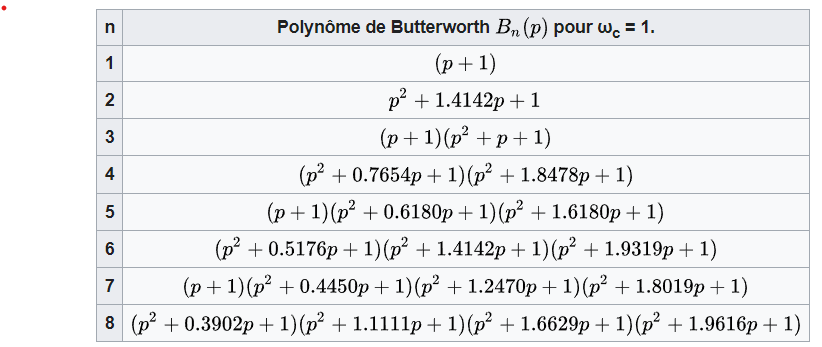
\includegraphics[width=12cm]{images/polynomes_butter.png}
\end{center}


La fonction de transfert normalisée s'écrit alors ($n$ impair et $n$ pair) :

$$ T(p) = \frac{1}{(1 + p) \cdot (a^2 + b^2 + 2\cdot b p + p^2) \cdot (...} \qquad  T(p) = \frac{1}{(a^2 + b^2 + 2\cdot b p + p^2) \cdot (...} $$

\end {document}